% !TEX root = ba_doc.tex
\begin{markdown}
\section{Feedback} \label{results}

To distribute our application and receive user feedback, we demonstrated our application to random students on the School Of Engineering campus. We asked the students to use our application for a bit and then fill out a survey. The survey contained questions about the usefulness, performance and design of ZHAWo as well as open questions about general feedback and improvement ideas. Out of 37 total survey participants, 76\% (28) rated the usefulness of ZHAWo with 5 out of 5 points (Figure \ref{fig:BarUsefulness}) and the average rating of the usefulness with 4.75 out of 5 was very high. The performance was rated with an average of 4.62 out of 5 points (Figure \ref{fig:BarPerformance}). The design of the application was rated with a lower point score of on average 4.24 out of 5 points (Figure \ref{fig:BarDesign}). The design rating is rather subjective, with some participants pointing out that they much prefer the simplistic design of ZHAWo over the official applications, while others list the design as an area where ZHAWo could improve a lot. Some of the lower ratings for the design can be attributed to the fact that especially on Huawei phones, the floor plans were not always displayed correctly.

In general, the room search feature and it's implementation with floor plans that display the locations of free rooms was received very positively, with most participants pointing out that feature as very useful and something they had been wishing for. A few participants also asked if the room search could be expanded to allow them to search for free rooms on a specific date. Others said that it should be expanded to also include other locations and not just the School Of Engineering campus at the Technikum.

The way we handled the display of overlapping events for timetables was also well received and was noted to be more readable compared to the official CampusInfo app.

In addition to getting feedback on our application, we also wanted to get a sense of how familiar people are with the concept of Progressive Web Applications. A majority of the survey participants (78\%) have not previously heard about PWAs. This coincided with what expected. PWAs are a new technology and people are only just starting to learn about them. 

\newpage

\begin{figure}[H]
  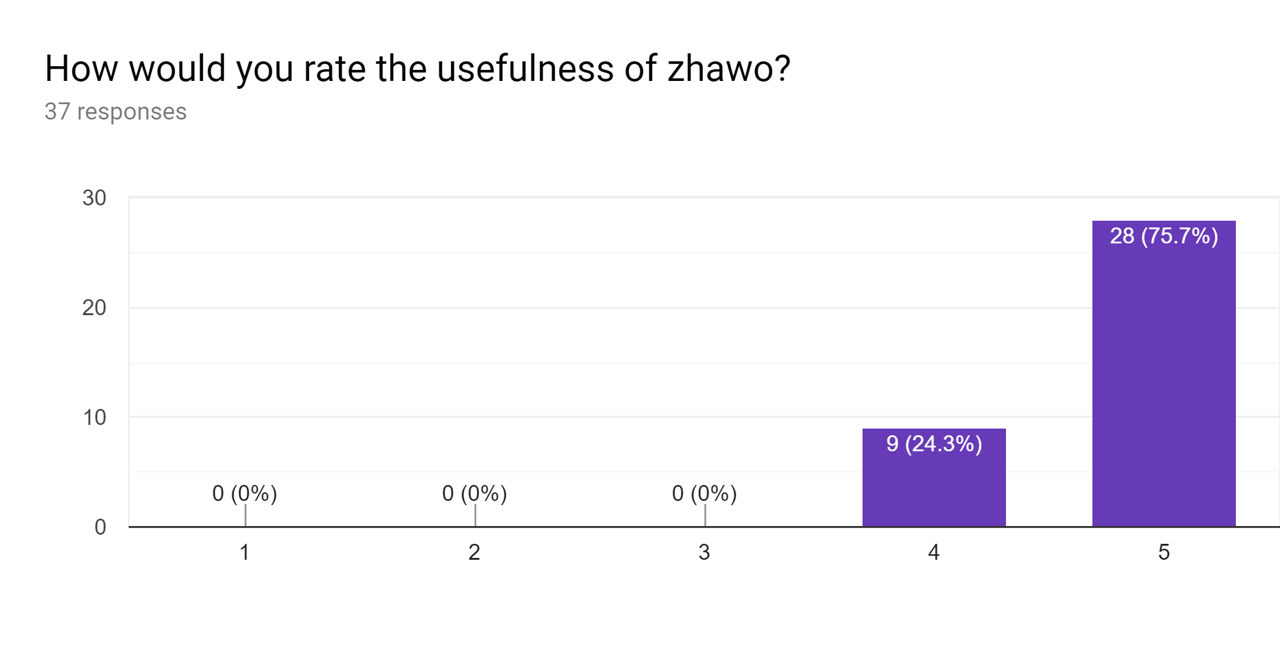
\includegraphics[width=13cm, center]{./figures/bar_1.png}
  \captionsetup{width=15.5cm}
  \caption [Usefulness Bar Diagram]{Distribution of the responses regarding the usefulness of ZHAWo.}
  \label{fig:BarUsefulness}
\end{figure}

\vspace{-5ex} % used to reduce padding after figure

\begin{figure}[H]
  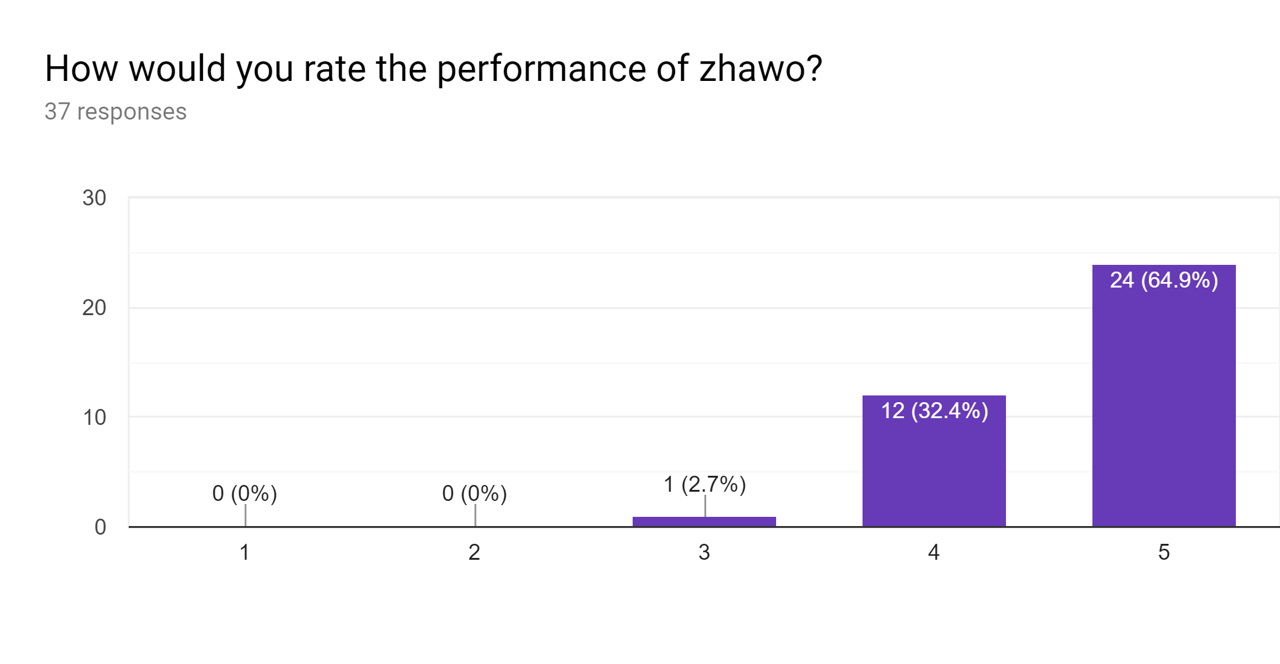
\includegraphics[width=13cm, center]{./figures/bar_2.png}
  \captionsetup{width=15.5cm}
  \caption [Performance Bar Diagram]{Distribution of the responses regarding the performance of ZHAWo.}
  \label{fig:BarPerformance}
\end{figure}

\vspace{-5ex} % used to reduce padding after figure

\begin{figure}[H]
  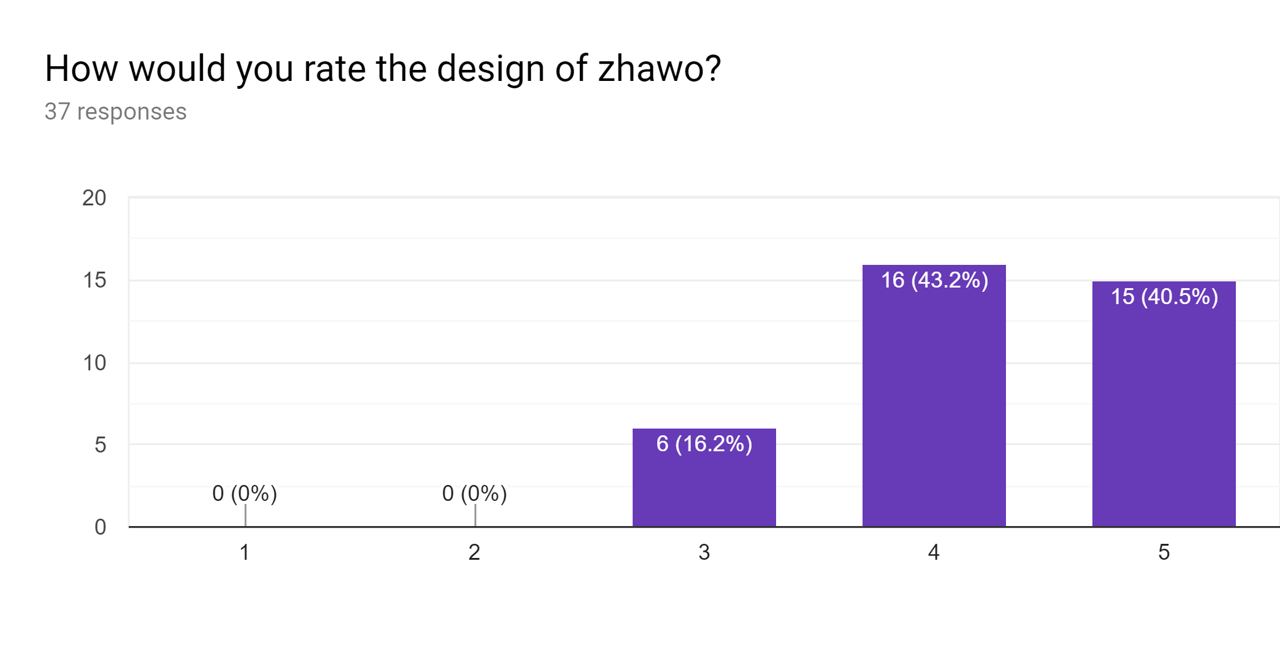
\includegraphics[width=13cm, center]{./figures/bar_3.png}
  \captionsetup{width=15.5cm}
  \caption [Design Bar Diagram]{Distribution of the responses regarding the design of ZHAWo.}
  \label{fig:BarDesign}
\end{figure}

\end{markdown}